\documentclass[10pt,a4paper,oneside]{beamer}
\usepackage[utf8]{inputenc}
\usepackage[ngerman]{babel}
\usepackage{amsmath}
\usepackage{amsfonts}
\usepackage{amssymb}
\usepackage{graphicx}
\usepackage{hyperref}
\usepackage{listings}
\usepackage{enumitem}
\author{Sabine Loch\and Matthias Jakobi}
\title{Basiswissen E-Mail\\ \small Thunderbird, SquirrelMail und E-Mail-Verteiler}
\usepackage{tikz}
\usepackage{environ}
\usepackage{sidecap}
\usepackage{wrapfig}
\usepackage{subfigure}
\usepackage{csquotes}
%\usepackage{mbox}

\makeatletter
\newsavebox{\measure@tikzpicture}
\NewEnviron{scaletikzpicturetowidth}[1]{%
    \def\tikz@width{#1}%
    \def\tikzscale{1}\begin{lrbox}{\measure@tikzpicture}%
        \BODY
    \end{lrbox}%
    \pgfmathparse{#1/\wd\measure@tikzpicture}%
    \edef\tikzscale{\pgfmathresult}%
    \BODY
}
\NewEnviron{scaletikzpicturetoheight}[1]{%
    \def\tikz@width{#1}%
    \def\tikzscale{1}\begin{lrbox}{\measure@tikzpicture}%
        \BODY
    \end{lrbox}%
    \pgfmathparse{#1/\ht\measure@tikzpicture}%
    \edef\tikzscale{\pgfmathresult}%
    \BODY
}
\makeatother

\definecolor{htworange}{HTML}{F4A621}
\definecolor{sturadarkgray}{HTML}{DDDDDD}
\definecolor{sturagray}{HTML}{EEEEEE}
                                    % Logo mit TikZ
\newcommand{\Logohtw}{
    \begin{tikzpicture}[scale=\tikzscale]
        \draw[black,fill=black] (0,0) -- (0,146) -- (29.5,146) -- (29.5,76) -- (88.5,76) -- (88.5,146) -- (159,146) -- (159,0) -- (130,0) -- (130,140) -- (94.5,140) -- (94.5,0) -- (88.5,0) -- (88.5,70) -- (29.5,70) -- (29.5,0) -- cycle;
        \draw[black,fill=black] (189,0) -- (189,146) -- (233,146) -- (233,140) -- (195,140) -- (195,10.5) -- (271.5,146) -- (303,146) -- (220.5,0) -- cycle;
        \draw[htworange,fill=htworange] (253.5,0) -- (336,146) -- (367,146) -- (285.5,0) -- cycle;
    \end{tikzpicture}
}

\newcommand{\LogoStuRaHTW}{
    \scalebox{.11}{
    % Created by Eps2pgf 0.7.0 (build on 2008-08-24) on Fri Mar 04 12:28:07 CET 2016
\begin{pgfpicture}
\pgfpathmoveto{\pgfqpoint{-0.002cm}{-0.002cm}}
\pgfpathlineto{\pgfqpoint{30.002cm}{-0.002cm}}
\pgfpathlineto{\pgfqpoint{30.002cm}{6.213cm}}
\pgfpathlineto{\pgfqpoint{-0.002cm}{6.213cm}}
\pgfpathclose
\pgfusepath{clip}
\begin{pgfscope}
\begin{pgfscope}
\end{pgfscope}
\begin{pgfscope}
\pgfpathmoveto{\pgfqpoint{0cm}{0cm}}
\pgfpathlineto{\pgfqpoint{30cm}{0cm}}
\pgfpathlineto{\pgfqpoint{30cm}{6.211cm}}
\pgfpathlineto{\pgfqpoint{0cm}{6.211cm}}
\pgfpathclose
\pgfusepath{clip}
\definecolor{eps2pgf_color}{rgb}{0.039216,0.039216,0.082353}\pgfsetstrokecolor{eps2pgf_color}\pgfsetfillcolor{eps2pgf_color}
\pgfpathmoveto{\pgfqpoint{20.133cm}{6.211cm}}
\pgfpathlineto{\pgfqpoint{17.525cm}{1.952cm}}
\pgfpathlineto{\pgfqpoint{16.25cm}{1.952cm}}
\pgfpathlineto{\pgfqpoint{18.858cm}{6.211cm}}
\pgfpathlineto{\pgfqpoint{20.133cm}{6.211cm}}
\pgfpathclose
\pgfpathmoveto{\pgfqpoint{17.525cm}{1.952cm}}
\pgfpathlineto{\pgfqpoint{17.091cm}{1.243cm}}
\pgfpathlineto{\pgfqpoint{15.814cm}{1.243cm}}
\pgfpathlineto{\pgfqpoint{16.249cm}{1.952cm}}
\pgfpathlineto{\pgfqpoint{17.525cm}{1.952cm}}
\pgfpathclose
\pgfpathmoveto{\pgfqpoint{16.306cm}{6.211cm}}
\pgfpathlineto{\pgfqpoint{13.697cm}{1.952cm}}
\pgfpathlineto{\pgfqpoint{12.422cm}{1.952cm}}
\pgfpathlineto{\pgfqpoint{15.03cm}{6.211cm}}
\pgfpathlineto{\pgfqpoint{16.306cm}{6.211cm}}
\pgfpathclose
\pgfpathmoveto{\pgfqpoint{13.698cm}{1.952cm}}
\pgfpathlineto{\pgfqpoint{13.263cm}{1.243cm}}
\pgfpathlineto{\pgfqpoint{11.987cm}{1.243cm}}
\pgfpathlineto{\pgfqpoint{12.422cm}{1.952cm}}
\pgfpathlineto{\pgfqpoint{13.698cm}{1.952cm}}
\pgfpathclose
\pgfpathmoveto{\pgfqpoint{17.092cm}{1.243cm}}
\pgfpathlineto{\pgfqpoint{16.872cm}{0.889cm}}
\pgfpathcurveto{\pgfqpoint{16.839cm}{0.829cm}}{\pgfqpoint{16.638cm}{0.592cm}}{\pgfqpoint{16.59cm}{0.534cm}}
\pgfpathlineto{\pgfqpoint{11.623cm}{0.534cm}}
\pgfpathcurveto{\pgfqpoint{11.65cm}{0.592cm}}{\pgfqpoint{11.734cm}{0.829cm}}{\pgfqpoint{11.768cm}{0.889cm}}
\pgfpathlineto{\pgfqpoint{11.987cm}{1.243cm}}
\pgfpathlineto{\pgfqpoint{17.092cm}{1.243cm}}
\pgfpathclose
\pgfpathmoveto{\pgfqpoint{16.59cm}{0.534cm}}
\pgfpathcurveto{\pgfqpoint{16.225cm}{0.178cm}}{\pgfqpoint{15.854cm}{0cm}}{\pgfqpoint{15.481cm}{0cm}}
\pgfpathlineto{\pgfqpoint{12.078cm}{0cm}}
\pgfpathcurveto{\pgfqpoint{11.704cm}{0cm}}{\pgfqpoint{11.552cm}{0.178cm}}{\pgfqpoint{11.623cm}{0.534cm}}
\pgfpathlineto{\pgfqpoint{16.59cm}{0.534cm}}
\pgfusepath{fill}
\definecolor{eps2pgf_color}{rgb}{0.933333,0.666667,0.223529}\pgfsetstrokecolor{eps2pgf_color}\pgfsetfillcolor{eps2pgf_color}
\pgfpathmoveto{\pgfqpoint{24.988cm}{4.969cm}}
\pgfpathlineto{\pgfqpoint{24.66cm}{4.437cm}}
\pgfpathcurveto{\pgfqpoint{24.621cm}{4.377cm}}{\pgfqpoint{24.414cm}{4.141cm}}{\pgfqpoint{24.371cm}{4.083cm}}
\pgfpathlineto{\pgfqpoint{23.163cm}{4.083cm}}
\pgfpathlineto{\pgfqpoint{23.711cm}{4.969cm}}
\pgfpathlineto{\pgfqpoint{24.988cm}{4.969cm}}
\pgfpathclose
\pgfpathmoveto{\pgfqpoint{23.611cm}{2.84cm}}
\pgfpathcurveto{\pgfqpoint{23.591cm}{2.781cm}}{\pgfqpoint{23.504cm}{2.545cm}}{\pgfqpoint{23.465cm}{2.486cm}}
\pgfpathlineto{\pgfqpoint{22.272cm}{0.534cm}}
\pgfpathlineto{\pgfqpoint{20.996cm}{0.534cm}}
\pgfpathlineto{\pgfqpoint{22.354cm}{2.84cm}}
\pgfpathlineto{\pgfqpoint{23.611cm}{2.84cm}}
\pgfpathclose
\pgfpathmoveto{\pgfqpoint{23.139cm}{1.952cm}}
\pgfpathlineto{\pgfqpoint{22.812cm}{1.421cm}}
\pgfpathlineto{\pgfqpoint{21.536cm}{1.421cm}}
\pgfpathlineto{\pgfqpoint{21.863cm}{1.952cm}}
\pgfpathlineto{\pgfqpoint{23.139cm}{1.952cm}}
\pgfpathclose
\pgfpathmoveto{\pgfqpoint{22.705cm}{1.243cm}}
\pgfpathlineto{\pgfqpoint{22.379cm}{0.712cm}}
\pgfpathlineto{\pgfqpoint{21.104cm}{0.712cm}}
\pgfpathlineto{\pgfqpoint{21.429cm}{1.243cm}}
\pgfpathlineto{\pgfqpoint{22.705cm}{1.243cm}}
\pgfpathclose
\pgfpathmoveto{\pgfqpoint{22.272cm}{0.534cm}}
\pgfpathlineto{\pgfqpoint{21.944cm}{0cm}}
\pgfpathlineto{\pgfqpoint{20.667cm}{0cm}}
\pgfpathlineto{\pgfqpoint{20.996cm}{0.534cm}}
\pgfpathlineto{\pgfqpoint{22.272cm}{0.534cm}}
\pgfpathclose
\pgfpathmoveto{\pgfqpoint{25.297cm}{5.501cm}}
\pgfpathlineto{\pgfqpoint{20.211cm}{5.501cm}}
\pgfpathlineto{\pgfqpoint{20.645cm}{6.211cm}}
\pgfpathlineto{\pgfqpoint{24.897cm}{6.211cm}}
\pgfpathcurveto{\pgfqpoint{25.272cm}{6.211cm}}{\pgfqpoint{25.509cm}{6.06cm}}{\pgfqpoint{25.297cm}{5.501cm}}
\pgfpathmoveto{\pgfqpoint{25.297cm}{5.501cm}}
\pgfpathcurveto{\pgfqpoint{25.27cm}{5.441cm}}{\pgfqpoint{25.237cm}{5.383cm}}{\pgfqpoint{25.2cm}{5.325cm}}
\pgfpathlineto{\pgfqpoint{24.987cm}{4.969cm}}
\pgfpathlineto{\pgfqpoint{19.883cm}{4.969cm}}
\pgfpathlineto{\pgfqpoint{20.211cm}{5.501cm}}
\pgfpathlineto{\pgfqpoint{25.297cm}{5.501cm}}
\pgfpathclose
\pgfpathmoveto{\pgfqpoint{21.16cm}{4.969cm}}
\pgfpathlineto{\pgfqpoint{20.61cm}{4.083cm}}
\pgfpathlineto{\pgfqpoint{19.335cm}{4.083cm}}
\pgfpathlineto{\pgfqpoint{19.883cm}{4.969cm}}
\pgfpathlineto{\pgfqpoint{21.16cm}{4.969cm}}
\pgfpathclose
\pgfpathmoveto{\pgfqpoint{24.371cm}{4.083cm}}
\pgfpathcurveto{\pgfqpoint{24.005cm}{3.727cm}}{\pgfqpoint{23.638cm}{3.55cm}}{\pgfqpoint{23.27cm}{3.55cm}}
\pgfpathlineto{\pgfqpoint{19.016cm}{3.55cm}}
\pgfpathlineto{\pgfqpoint{19.335cm}{4.083cm}}
\pgfpathlineto{\pgfqpoint{24.371cm}{4.083cm}}
\pgfpathclose
\pgfpathmoveto{\pgfqpoint{23.611cm}{2.84cm}}
\pgfpathlineto{\pgfqpoint{18.575cm}{2.84cm}}
\pgfpathlineto{\pgfqpoint{19.018cm}{3.558cm}}
\pgfpathlineto{\pgfqpoint{23.22cm}{3.55cm}}
\pgfpathcurveto{\pgfqpoint{23.595cm}{3.55cm}}{\pgfqpoint{23.682cm}{3.196cm}}{\pgfqpoint{23.611cm}{2.84cm}}
\pgfpathmoveto{\pgfqpoint{20.295cm}{3.558cm}}
\pgfpathlineto{\pgfqpoint{18.445cm}{0.534cm}}
\pgfpathlineto{\pgfqpoint{17.169cm}{0.534cm}}
\pgfpathlineto{\pgfqpoint{19.018cm}{3.558cm}}
\pgfpathlineto{\pgfqpoint{20.295cm}{3.558cm}}
\pgfpathclose
\pgfpathmoveto{\pgfqpoint{19.311cm}{1.952cm}}
\pgfpathlineto{\pgfqpoint{18.985cm}{1.421cm}}
\pgfpathlineto{\pgfqpoint{17.708cm}{1.421cm}}
\pgfpathlineto{\pgfqpoint{18.035cm}{1.952cm}}
\pgfpathlineto{\pgfqpoint{19.311cm}{1.952cm}}
\pgfpathclose
\pgfpathmoveto{\pgfqpoint{18.879cm}{1.243cm}}
\pgfpathlineto{\pgfqpoint{18.549cm}{0.712cm}}
\pgfpathlineto{\pgfqpoint{17.276cm}{0.712cm}}
\pgfpathlineto{\pgfqpoint{17.601cm}{1.243cm}}
\pgfpathlineto{\pgfqpoint{18.879cm}{1.243cm}}
\pgfpathclose
\pgfpathmoveto{\pgfqpoint{18.445cm}{0.534cm}}
\pgfpathlineto{\pgfqpoint{18.118cm}{0cm}}
\pgfpathlineto{\pgfqpoint{16.842cm}{0cm}}
\pgfpathlineto{\pgfqpoint{17.169cm}{0.534cm}}
\pgfpathlineto{\pgfqpoint{18.445cm}{0.534cm}}
\pgfusepath{fill}
\definecolor{eps2pgf_color}{rgb}{0.039216,0.039216,0.082353}\pgfsetstrokecolor{eps2pgf_color}\pgfsetfillcolor{eps2pgf_color}
\pgfpathmoveto{\pgfqpoint{28.579cm}{0cm}}
\pgfpathlineto{\pgfqpoint{27.134cm}{0cm}}
\pgfpathlineto{\pgfqpoint{27.458cm}{1.421cm}}
\pgfpathlineto{\pgfqpoint{28.902cm}{1.421cm}}
\pgfpathlineto{\pgfqpoint{28.579cm}{0cm}}
\pgfpathclose
\pgfpathmoveto{\pgfqpoint{29.679cm}{4.792cm}}
\pgfpathlineto{\pgfqpoint{26.974cm}{4.792cm}}
\pgfpathlineto{\pgfqpoint{28.384cm}{6.211cm}}
\pgfpathlineto{\pgfqpoint{30cm}{6.211cm}}
\pgfpathlineto{\pgfqpoint{29.679cm}{4.792cm}}
\pgfpathclose
\pgfpathmoveto{\pgfqpoint{29.185cm}{2.662cm}}
\pgfpathlineto{\pgfqpoint{27.739cm}{2.662cm}}
\pgfpathlineto{\pgfqpoint{28.177cm}{4.552cm}}
\pgfpathlineto{\pgfqpoint{26.294cm}{2.662cm}}
\pgfpathlineto{\pgfqpoint{24.848cm}{2.662cm}}
\pgfpathlineto{\pgfqpoint{26.974cm}{4.792cm}}
\pgfpathlineto{\pgfqpoint{29.679cm}{4.792cm}}
\pgfpathlineto{\pgfqpoint{29.185cm}{2.662cm}}
\pgfpathclose
\pgfpathmoveto{\pgfqpoint{29.064cm}{2.131cm}}
\pgfpathlineto{\pgfqpoint{24.317cm}{2.131cm}}
\pgfpathlineto{\pgfqpoint{24.848cm}{2.662cm}}
\pgfpathlineto{\pgfqpoint{29.185cm}{2.662cm}}
\pgfpathlineto{\pgfqpoint{29.064cm}{2.131cm}}
\pgfpathclose
\pgfpathmoveto{\pgfqpoint{28.902cm}{1.421cm}}
\pgfpathlineto{\pgfqpoint{23.612cm}{1.421cm}}
\pgfpathlineto{\pgfqpoint{24.317cm}{2.131cm}}
\pgfpathlineto{\pgfqpoint{29.064cm}{2.131cm}}
\pgfpathlineto{\pgfqpoint{28.902cm}{1.421cm}}
\pgfpathclose
\pgfpathmoveto{\pgfqpoint{25.057cm}{1.421cm}}
\pgfpathlineto{\pgfqpoint{23.646cm}{0cm}}
\pgfpathlineto{\pgfqpoint{22.2cm}{0cm}}
\pgfpathlineto{\pgfqpoint{23.612cm}{1.421cm}}
\pgfpathlineto{\pgfqpoint{25.057cm}{1.421cm}}
\pgfusepath{fill}
\pgfpathmoveto{\pgfqpoint{6.837cm}{2.84cm}}
\pgfpathlineto{\pgfqpoint{5.864cm}{1.243cm}}
\pgfpathlineto{\pgfqpoint{4.586cm}{1.243cm}}
\pgfpathlineto{\pgfqpoint{5.562cm}{2.84cm}}
\pgfpathlineto{\pgfqpoint{6.837cm}{2.84cm}}
\pgfpathclose
\pgfpathmoveto{\pgfqpoint{8.907cm}{6.211cm}}
\pgfpathlineto{\pgfqpoint{8.579cm}{5.679cm}}
\pgfpathlineto{\pgfqpoint{3.543cm}{5.679cm}}
\pgfpathcurveto{\pgfqpoint{3.909cm}{6.033cm}}{\pgfqpoint{4.28cm}{6.211cm}}{\pgfqpoint{4.652cm}{6.211cm}}
\pgfpathlineto{\pgfqpoint{8.907cm}{6.211cm}}
\pgfpathclose
\pgfpathmoveto{\pgfqpoint{8.579cm}{5.679cm}}
\pgfpathlineto{\pgfqpoint{8.145cm}{4.969cm}}
\pgfpathlineto{\pgfqpoint{3.042cm}{4.969cm}}
\pgfpathlineto{\pgfqpoint{3.254cm}{5.325cm}}
\pgfpathcurveto{\pgfqpoint{3.292cm}{5.383cm}}{\pgfqpoint{3.492cm}{5.619cm}}{\pgfqpoint{3.543cm}{5.679cm}}
\pgfpathlineto{\pgfqpoint{8.579cm}{5.679cm}}
\pgfpathclose
\pgfpathmoveto{\pgfqpoint{4.318cm}{4.969cm}}
\pgfpathlineto{\pgfqpoint{3.771cm}{4.083cm}}
\pgfpathlineto{\pgfqpoint{2.494cm}{4.083cm}}
\pgfpathlineto{\pgfqpoint{3.042cm}{4.969cm}}
\pgfpathlineto{\pgfqpoint{4.318cm}{4.969cm}}
\pgfpathclose
\pgfpathmoveto{\pgfqpoint{7.148cm}{3.373cm}}
\pgfpathlineto{\pgfqpoint{2.129cm}{3.373cm}}
\pgfpathcurveto{\pgfqpoint{2.15cm}{3.432cm}}{\pgfqpoint{2.243cm}{3.669cm}}{\pgfqpoint{2.282cm}{3.727cm}}
\pgfpathlineto{\pgfqpoint{2.494cm}{4.083cm}}
\pgfpathlineto{\pgfqpoint{6.747cm}{4.083cm}}
\pgfpathcurveto{\pgfqpoint{7.121cm}{4.083cm}}{\pgfqpoint{7.213cm}{3.728cm}}{\pgfqpoint{7.148cm}{3.373cm}}
\pgfpathmoveto{\pgfqpoint{7.148cm}{3.373cm}}
\pgfpathcurveto{\pgfqpoint{7.126cm}{3.313cm}}{\pgfqpoint{7.096cm}{3.254cm}}{\pgfqpoint{7.057cm}{3.196cm}}
\pgfpathlineto{\pgfqpoint{6.837cm}{2.84cm}}
\pgfpathlineto{\pgfqpoint{2.584cm}{2.84cm}}
\pgfpathcurveto{\pgfqpoint{2.215cm}{2.84cm}}{\pgfqpoint{2.064cm}{3.016cm}}{\pgfqpoint{2.129cm}{3.373cm}}
\pgfpathlineto{\pgfqpoint{7.148cm}{3.373cm}}
\pgfpathclose
\pgfpathmoveto{\pgfqpoint{5.864cm}{1.243cm}}
\pgfpathlineto{\pgfqpoint{5.644cm}{0.889cm}}
\pgfpathcurveto{\pgfqpoint{5.611cm}{0.829cm}}{\pgfqpoint{5.411cm}{0.592cm}}{\pgfqpoint{5.362cm}{0.534cm}}
\pgfpathlineto{\pgfqpoint{0.327cm}{0.534cm}}
\pgfpathlineto{\pgfqpoint{0.76cm}{1.243cm}}
\pgfpathlineto{\pgfqpoint{5.864cm}{1.243cm}}
\pgfpathclose
\pgfpathmoveto{\pgfqpoint{5.362cm}{0.534cm}}
\pgfpathcurveto{\pgfqpoint{4.996cm}{0.178cm}}{\pgfqpoint{4.626cm}{0cm}}{\pgfqpoint{4.252cm}{0cm}}
\pgfpathlineto{\pgfqpoint{0cm}{0cm}}
\pgfpathlineto{\pgfqpoint{0.327cm}{0.534cm}}
\pgfpathlineto{\pgfqpoint{5.362cm}{0.534cm}}
\pgfusepath{fill}
\pgfpathmoveto{\pgfqpoint{11.929cm}{4.976cm}}
\pgfpathlineto{\pgfqpoint{9.216cm}{0.534cm}}
\pgfpathlineto{\pgfqpoint{7.941cm}{0.534cm}}
\pgfpathlineto{\pgfqpoint{10.654cm}{4.976cm}}
\pgfpathlineto{\pgfqpoint{11.929cm}{4.976cm}}
\pgfpathclose
\pgfpathmoveto{\pgfqpoint{9.216cm}{0.534cm}}
\pgfpathlineto{\pgfqpoint{8.889cm}{0cm}}
\pgfpathlineto{\pgfqpoint{7.612cm}{0cm}}
\pgfpathlineto{\pgfqpoint{7.941cm}{0.534cm}}
\pgfpathlineto{\pgfqpoint{9.216cm}{0.534cm}}
\pgfpathclose
\pgfpathmoveto{\pgfqpoint{14.519cm}{6.211cm}}
\pgfpathlineto{\pgfqpoint{14.085cm}{5.501cm}}
\pgfpathlineto{\pgfqpoint{8.982cm}{5.501cm}}
\pgfpathlineto{\pgfqpoint{9.416cm}{6.211cm}}
\pgfpathlineto{\pgfqpoint{14.519cm}{6.211cm}}
\pgfpathclose
\pgfpathmoveto{\pgfqpoint{14.086cm}{5.501cm}}
\pgfpathlineto{\pgfqpoint{13.759cm}{4.969cm}}
\pgfpathlineto{\pgfqpoint{8.655cm}{4.969cm}}
\pgfpathlineto{\pgfqpoint{8.982cm}{5.501cm}}
\pgfpathlineto{\pgfqpoint{14.086cm}{5.501cm}}
\pgfusepath{fill}
\end{pgfscope}
\end{pgfscope}
\end{pgfpicture}

    }
}


\setbeamertemplate{headline}
{
    \leavevmode%
    \hbox{%
        \begin{beamercolorbox}[wd=\paperwidth,ht=9.5ex,dp=1ex]{secsubsec}%
            {   \LogoStuRaHTW{}}
            \hspace*{38em}%
            {
                \begin{scaletikzpicturetowidth}{0.13\textwidth}
                    \Logohtw{}
                \end{scaletikzpicturetowidth}
            }
            %
        \end{beamercolorbox}%
    }%
}
\setbeamercolor{secsubsec}{bg=sturadarkgray}
%\setbeamercolor{background canvas}{bg=sturagray}
\setbeamercolor{frametitle}{fg=htworange}
\setbeamercolor{item}{fg=htworange}
\setbeamercolor{structure}{fg=htworange}
%\setbeamercolor{palette sidebar}{fg=red}
%\beamertemplatenavigationsymbolsempty
\setbeamertemplate{footline}[frame number]
\setitemize{label=\usebeamerfont*{itemize item}%
      \usebeamercolor[fg]{itemize item}
        \usebeamertemplate{itemize item}}

%\addtobeamertemplate{frametitle}{\vskip+3.7ex}{}
\newcommand{\secframe}[2]{
\section{#1}
\frame{
        \frametitle{#1}
        {#2}
}
}
\newcommand{\subsecframe}[2]{
\subsection{#1}
\frame{
        \frametitle{#1}
        {#2}
}
}
\setcounter{tocdepth}{1}
\AtBeginSection[]
{
  \begin{frame}
    \frametitle{Inhaltsverzeichnis}
    \tableofcontents[currentsection]
  \end{frame}
}


\newlist{tip}{enumerate}{1}
\setlist[tip]{label=Tipp: ,leftmargin=*}

\newlist{hinweis}{enumerate}{1}
\setlist[hinweis]{label=Hinweis: ,leftmargin=*}

\lstset{
    frame=tb, % draw a frame at the top and bottom of the code block
    tabsize=2, % tab space width
    showstringspaces=false, % don't mark spaces in strings
    numbers=left, % display line numbers on the left
    commentstyle=\color{green}, % comment color
    keywordstyle=\color{blue}, % keyword color
    stringstyle=\color{red} % string color
}
\hypersetup{
    colorlinks=true,
    linkcolor=blue,
    urlcolor=red,
    linktoc=all
}

\begin{document}
\maketitle
\frame{\frametitle{Inhaltsverzeichnis}\tableofcontents}


\secframe{Schreiben von E-Mails}{
	Was beim Schreiben einer E-Mail zu beachten ist.
	\begin{itemize}
		\item Betreff \textbf{nicht} aussschlie{\ss}lich mit \MakeUppercase{Gro{\ss}buchstaben}
		\item Satzzeichen sind keine Rudeltiere!\textbf{(!!)}
		\item Rechtschreibkorrektur verwenden
		\item StuRa E-Mail Adresse verwenden
		\item Relevante Personen und/oder Verteiler in Kopie (CC) setzen
	\end{itemize}

}
\secframe{Allgemein}{
	Die StuRa E-Mail Adresse bildet sich aus eurem Nachnamen \texttt{nachname@stura.htw-dresden.de} und ist eine \textbf{Weiterleitung} auf euer HTW-Postfach.
Daher ben\"otigt Ihr lediglich euren Hochschulzugang:
	\begin{itemize}
		\item S-Nummer
		\item Hochschulpassword
	\end{itemize}
	Falls die E-Mail Adresse bereits vergeben ist, werden solange die Anfangsbuchstaben des Vornamen als Pr\"afix aufgef\"ullt, bis die Adresse einzigartig ist.
	\begin{hinweis}
    \item Eine Weiterleitung der StuRa-Adressen auf private E-Mail Konten wird \emph{nicht empfohlen}.
	\end{hinweis}
	\begin{tip}
	\item Bei niedrigem Speicherplatz kann über den Service des Rechenzentrums eine Erh\"ohung veranlasst werden.
	\end{tip}
}

\secframe{SquirrelMail}{
	Web-Adressen f\"ur den Webmailer.
	\begin{description}
		\item[allg.] \url{https://webmail.htw-dresden.de}
		\item[Info/Mathe] \url{https://webmail.informatik.htw-dresden.de}
		\item[WiWi] \url{https://webmail.wiwi.htw-dresden.de}
	\end{description}
   \begin{figure}
	   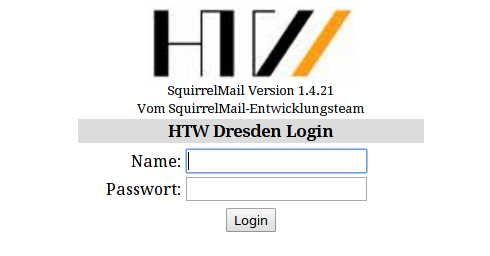
\includegraphics[width=0.7\textwidth]{../images/wm_loginseite.png}
   \end{figure}
}

\frame{
	\frametitle{SquirrelMail Startseite}
	Nach dem Login erh\"alt man eine \"Ubersicht der empfangen Mails und kann im oberen Bereich folgende Funktionen w\"ahlen:
	\begin{description}
		\item[Verfassen] E-Mail schreiben
		\item[Adressen]
		\item[Ordner] erstellen/umbenennen/l\"oschen/austragen der eintragen
		\item[Optionen] Manage Identities/Farbthema
		\item[Suchen]
		\item[Hilfe]
		\item[Filter] Filterregeln (de)aktivieren/erstellen
		\item[Kalender]
	\end{description}
	}
\frame{
	\frametitle{SquirrelMail Startseite II}
   \begin{figure}
	   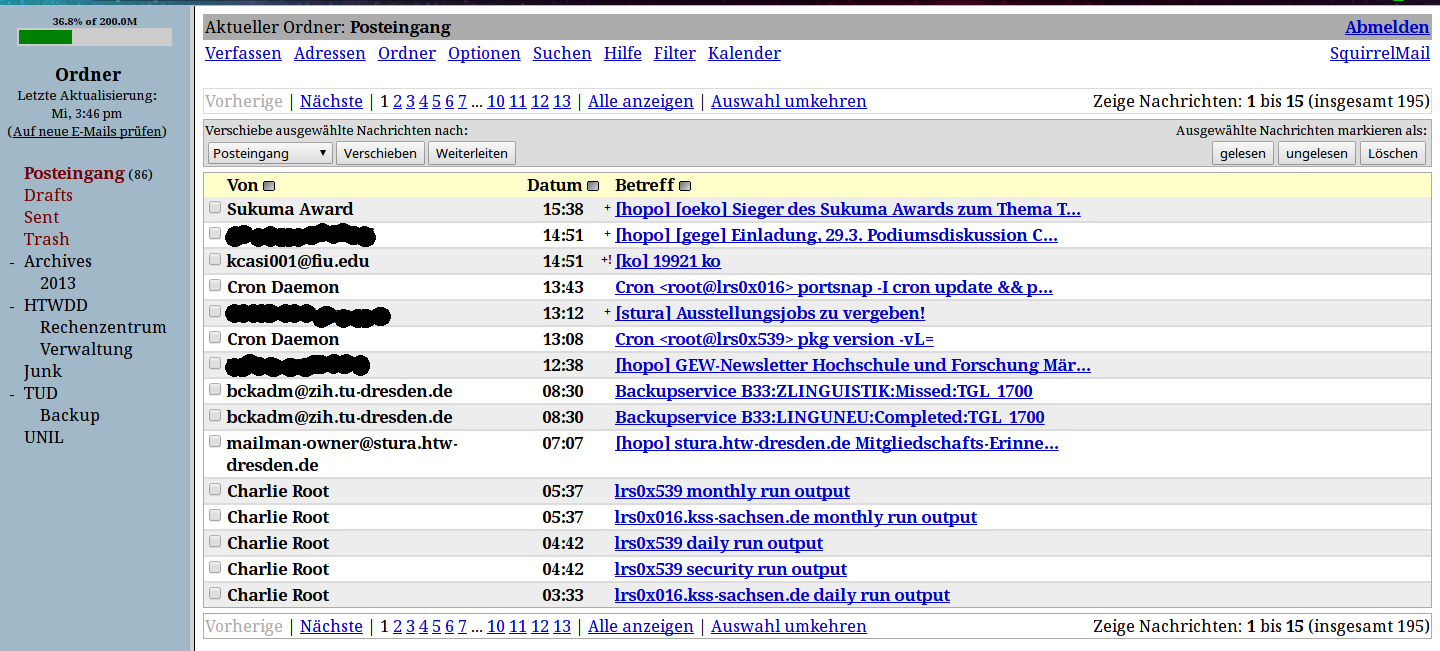
\includegraphics[width=\textwidth]{../images/wm_startseite.png}
   \end{figure}
}
\subsecframe{Ordner}{
	\begin{itemize}
		\item erstellen
		\item umbenennen
		\item l\"oschen
		\item austragen/eintragen
	\end{itemize}
	}
\frame{
	\frametitle{Ordner II}
   \begin{figure}
	   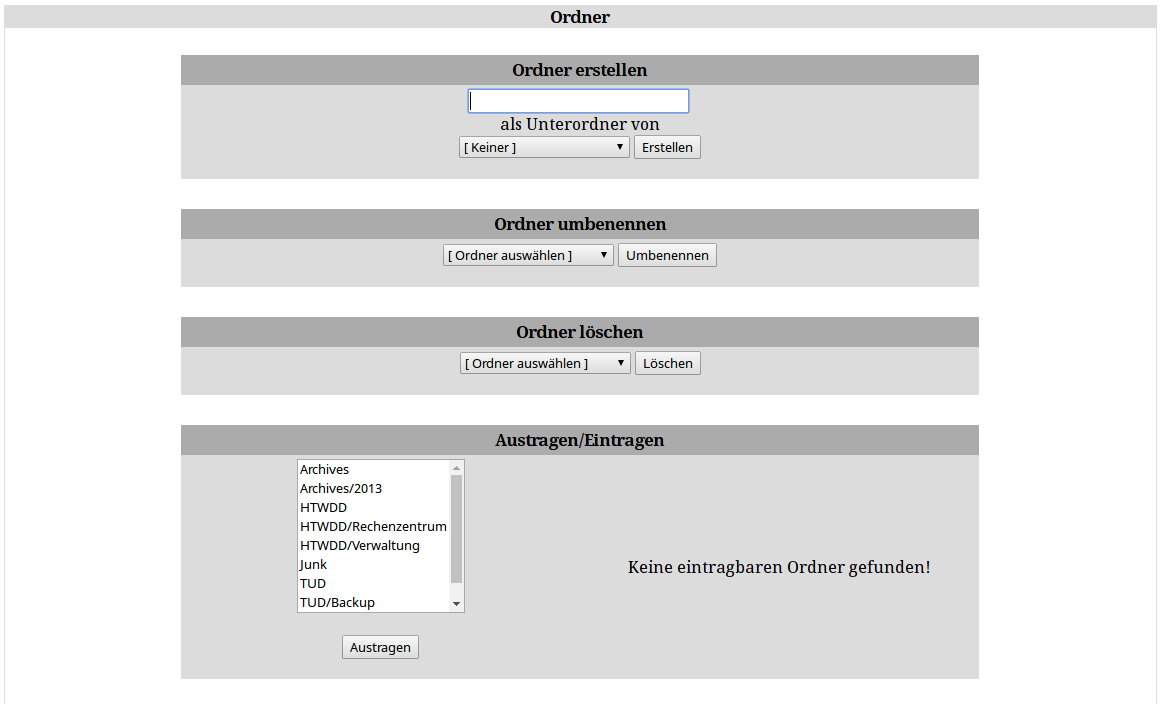
\includegraphics[width=\textwidth]{../images/wm_ordner.png}
   \end{figure}
}

\subsecframe{Optionen}{
	Manage Identities / Aliases
	}

\subsecframe{Filter} {
	\begin{itemize}
		\item aktivieren
		\item deaktivieren
		\item hinzuf\"ugen
		\item bearbeiten/kopieren/l\"oschen
	\end{itemize}
   \begin{figure}
	   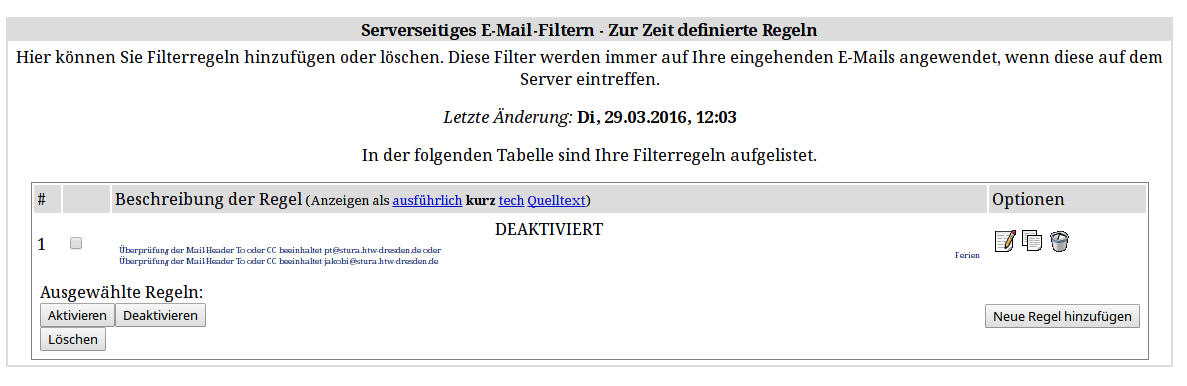
\includegraphics[width=\textwidth]{../images/wm_filterseite.png}
   \end{figure}
}

\frame{
	\frametitle{Filter II}
   \begin{figure}
	   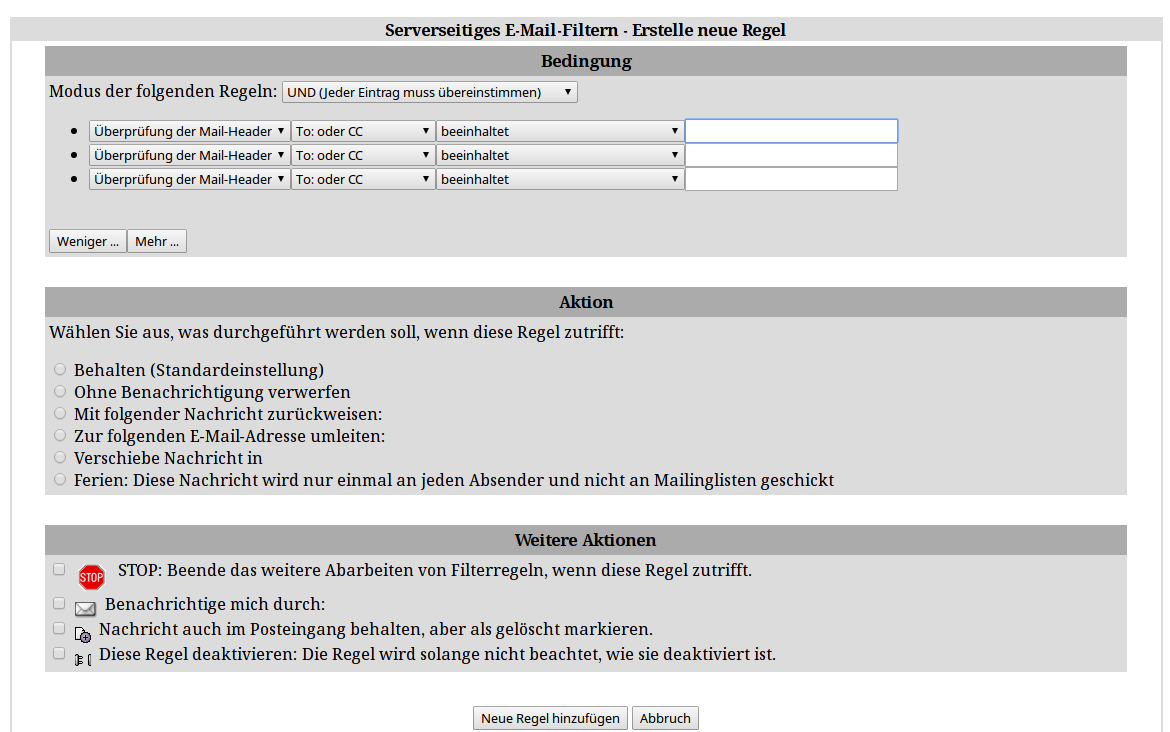
\includegraphics[width=\textwidth]{../images/wm_neue_filter_regeln.png}
   \end{figure}
}

%Webmailer
%%%webmailer url

\secframe{Thunderbird}{
	Thunderbird\footnote{\url{https://mozilla.org/thunderbird}} ist ein E-Mail Client von Mozilla
	und f\"ur die g\"angigen Betriebssysteme verf\"ugbar.
	
	Es gibt weitere E-Mail Clients wie KMail, Evolution, Mutt und so weiter.
}

\subsecframe{Zugriff}{
	Um einen E-Mail Client einzurichten, empfiehlt es sich im Hochschulnetzwerk
	mit seinem Laptop oder im VPN mit seinem Heimrechner zu sein.
	\begin{tip}
    \item Zum Einrichten einer VPN Verbindung siehe die Anleitung des Rechenzentrums\footnote{\url{https://www.htw-dresden.de/rz/vpn}}.
	\end{tip}
}

\subsecframe{Konto einrichten}{
	Zur Einrichtung des E-Mail Kontos ben\"otigt man
	\begin{itemize}
		\item S-Nummer und
		\item Hochschulpassword.
	\end{itemize}
In einigen F\"allen ist es sinnvoll Informationen \"uber den Mail-Server des RZ\footnote{\url{https://www.htw-dresden.de/rz/zentrale-dienste-und-server/e-mail-an-der-htw.html}} zu haben.
	\begin{itemize}
		\item Incoming
	\begin{description}
		\item[Server hostname] imap.htw-dresden.de
		\item[Port] 143
		\item[SSL] STARTTLS
		\item[Authentication] Normal password
	\end{description}
		\item Outgoing
	\begin{description}
		\item[Server hostname] mail.htw-dresden.de
		\item[Port] 25
		\item[SSL] STARTTLS
		\item[Authentication] Normal password
	\end{description}
	\end{itemize}
}

\frame{
    \frametitle{Konto einrichten II}
    \begin{columns}
        \begin{column}{0.5\textwidth}
            \begin{figure}[!h]
                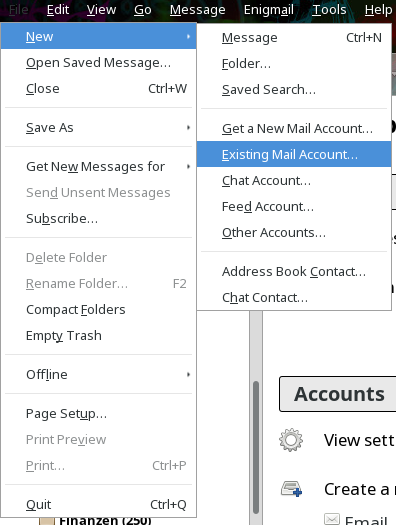
\includegraphics[width=0.7\textwidth]{../images/tb_new_mail_account.png}
            \end{figure}
        \end{column}
        \begin{column}{0.5\textwidth}
            \begin{description}
                \item[1.] File/Datei
                \item[2.] New/Neu
                \item[3.] Exisiting Mail account/ Mail-Konto
            \end{description}
        \end{column}
    \end{columns}
}

\frame{
	\frametitle{Konto einrichten III}
	 \begin{figure}[!h]
		 \centering
		 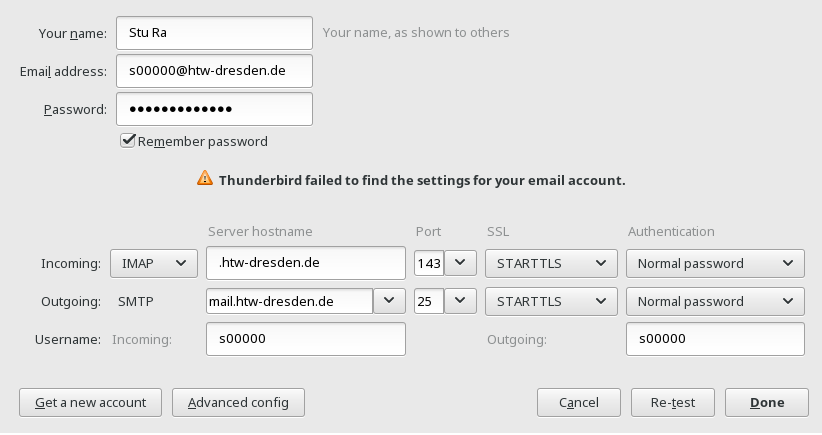
\includegraphics[width=0.9\textwidth]{../images/tb_new_mail_account_II.png}
		 \vspace{-20pt}
	 \end{figure}
 }

\subsecframe{Ordner anlegen}{
	\begin{minipage}[b]{0.35\linewidth}
		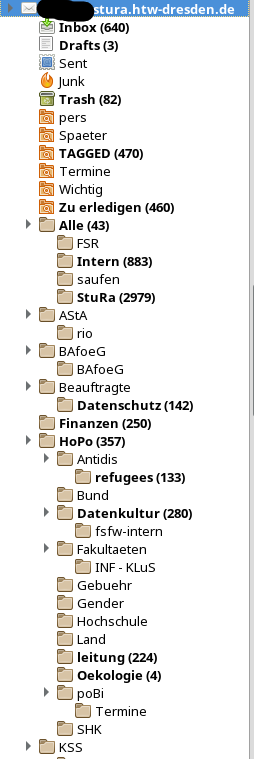
\includegraphics[height=0.8\textheight]{../images/tb_filestruct.png}
	\end{minipage}
	\begin{minipage}[t]{0.63\linewidth}
		\vspace{-5cm}
		\large
	Das Erstellen von Ordnern hilft bei der Klassifizierung und Sortierung der erhaltenen e-Mails.
	\end{minipage}
}

\frame{
	\frametitle{Ordner anlegen II}
	   \begin{figure}
	   \subfigure[Ordner anlegen] {
		   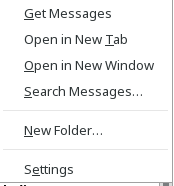
\includegraphics[height=0.5\textheight]{../images/tb_new_folder_I.png}
		   }
	   \subfigure[Unterordner anlegen] {
		   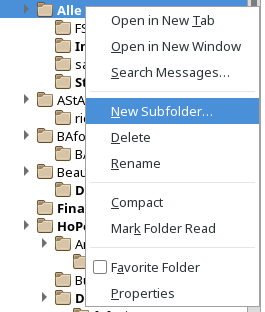
\includegraphics[height=0.5\textheight]{../images/tb_new_subfolder_I.png}
		   }
	   \end{figure}
	   \textit{Rechtsklick} $->$ New Folder oder New Subfolder
   }

\frame{
	\frametitle{Ordner anlegen III}
	   \begin{figure}
		   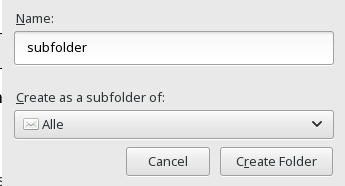
\includegraphics[height=0.5\textheight]{../images/tb_new_subfolder_II.png}
	   \end{figure}
	\begin{description}
		\item[Name:] Name des Ordners
		\item[Create as a subfolder of:] Erstelle als Unterordner von:
	\end{description}
	}

\subsecframe{Manage Identities / Aliases}{
	Accounts $->$ View settings for this account $->$ Manage Identities $->$ Add
	Konten $->$ Zeige Kontoeinstellungen $->$ 
   \begin{figure}
	   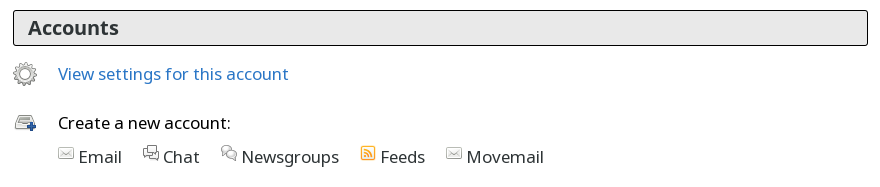
\includegraphics[width=\textwidth]{../images/tb_accounts.png}
   \end{figure}
}

\frame {
    \frametitle{Manage Identities / Aliases II}
    \begin{columns}
        \begin{column}{0.5\textwidth}
            \begin{figure}
                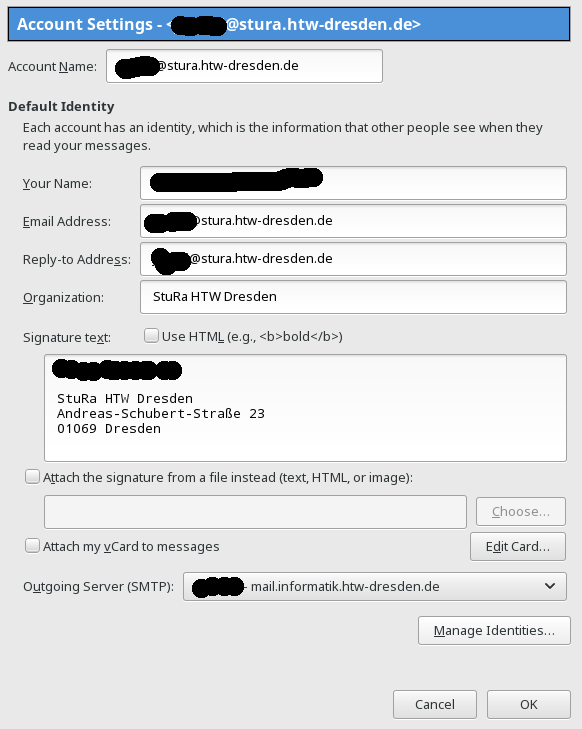
\includegraphics[width=\textwidth]{../images/tb_account_settings.png}
            \end{figure}
        \end{column}
        \begin{column}{0.53\textwidth}  %%<--- here
            \begin{description}
                \item[Account Name:] frei w\"ahlbar
                \item[Your Name:] Vorname Nachname
                \item[Email Address:] \texttt{nachname@stura.htw-dresden.de}
                \item[Replay-To Address:] selbe wie Email Adresse
                \item[Organization:] StuRa HTW Dresden
                \item[Signature text:] Vorname Nachname\newline
                    \newline
                    StuRa HTW Dresden\newline
                    Andreas-Schubert-Str. 23\newline
                    01069 Dresden
                \item[Outgoing Server (SMTP):] mail.htw-dresden.de
            \end{description}
        \end{column}
    \end{columns}
}

\frame {
	\frametitle{Manage Identities / Aliases III}
   \begin{figure}
	   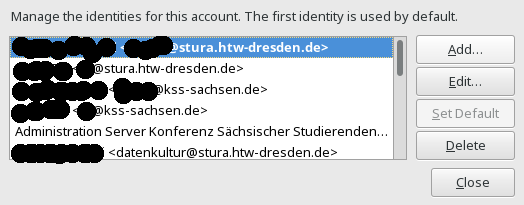
\includegraphics[width=\textwidth]{../images/tb_manage_identities.png}
   \end{figure}
   Es ist praktisch Aliases f\"ur die Bereiche und Referate zuerstellen.
}

\frame {
	\frametitle{Manage Identities / Aliases IV}

    \begin{columns}
        \begin{column}{0.5\textwidth}
            \begin{figure}
                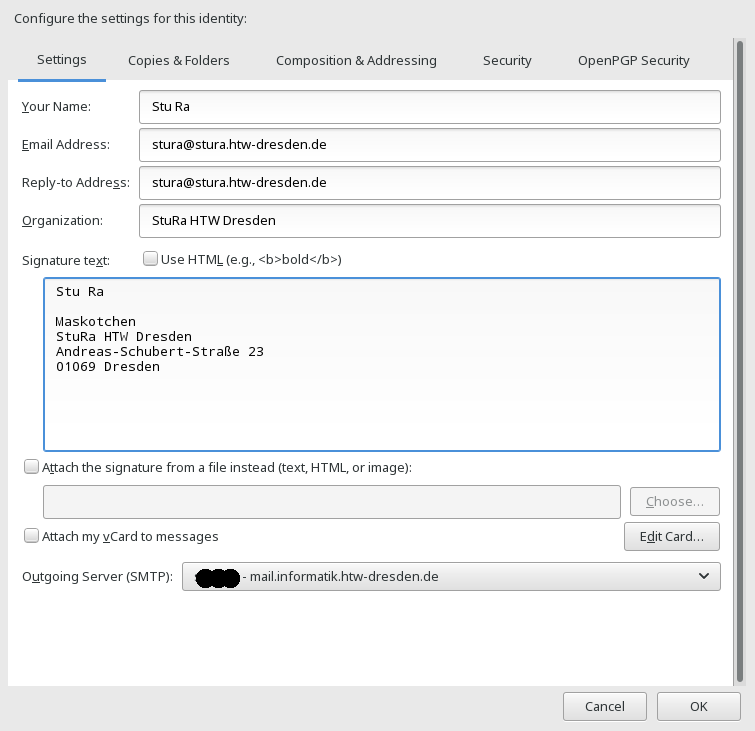
\includegraphics[width=\textwidth]{../images/tb_add_identitie.png}
            \end{figure}
        \end{column}
        \begin{column}{0.53\textwidth}  %%<--- here
            \begin{description}
                \item[Account Name:] frei w\"ahlbar
                \item[Your Name:] Funktion
                \item[Email Address:] \texttt{funktion@stura.htw-dresden.de}
                \item[Replay-To Address:] selbe wie Email Adresse
                \item[Organization:] StuRa HTW Dresden
                \item[Signature text:] Funktion\newline
                    \newline
                    StuRa HTW Dresden\newline
                    Andreas-Schubert-Str. 23\newline
                    01069 Dresden
                \item[Outgoing Server (SMTP):] mail.htw-dresden.de
            \end{description}
        \end{column}
    \end{columns}
}

\subsecframe{Filter} {
   \begin{figure}
	   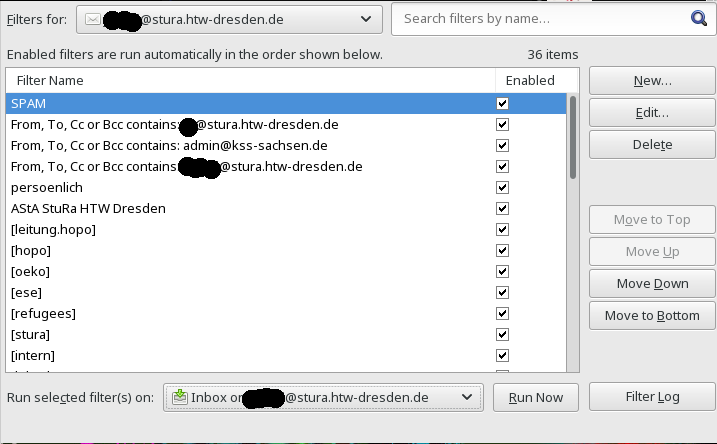
\includegraphics[height=0.8\textheight]{../images/tb_message_filters.png}
   \end{figure}
	
}

\frame {
	\frametitle{Filter II}
   \begin{figure}
	   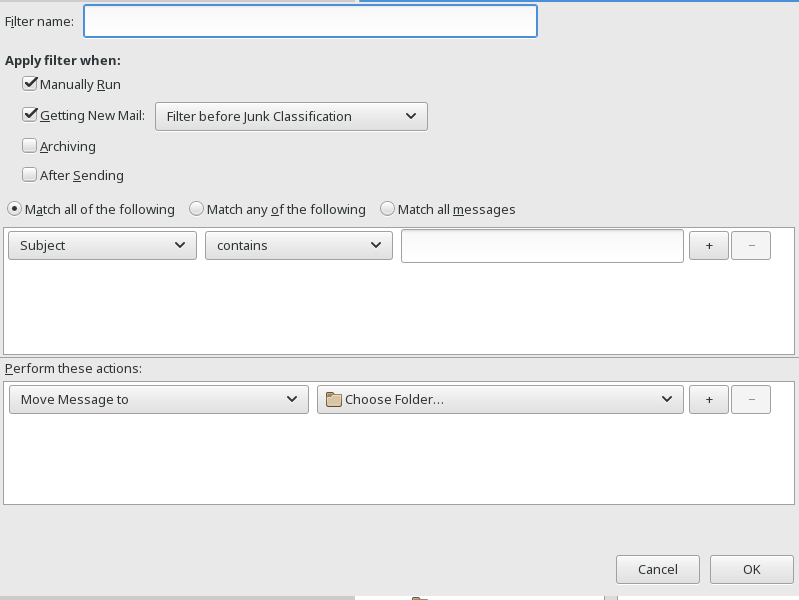
\includegraphics[height=0.8\textheight]{../images/tb_new_filter_rules.png}
   \end{figure}

}
\frame{
	\frametitle{Spamfilter}
   \begin{figure}
	   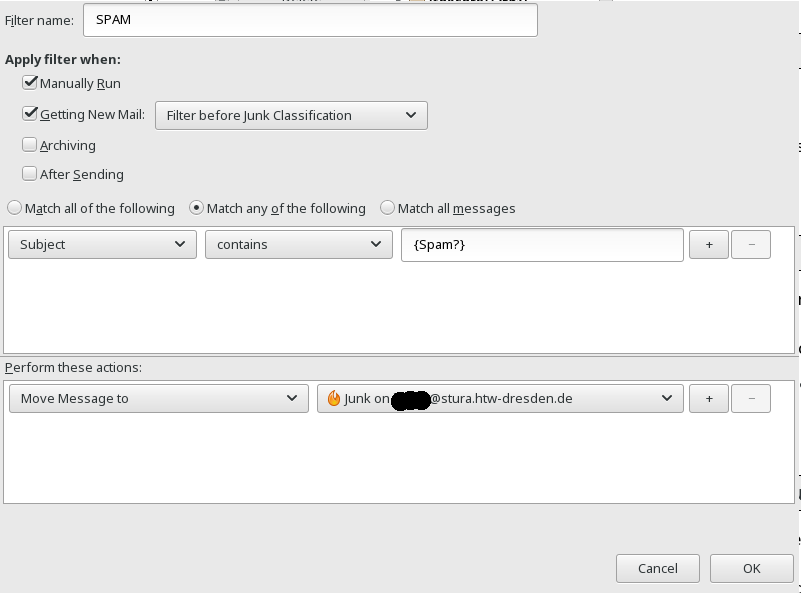
\includegraphics[height=0.8\textheight]{../images/tb_new_spam_filter_rule.png}
   \end{figure}
}
%%%spamfilter
%%%sortieren

\secframe{StuRa E-Mail-Verteiler} {
	Web-Adresse f\"ur die \"Ubersicht der E-Mail-Verteiler vom StuRa \url{https://lists.stura.htw-dresden.de}.
   \begin{figure}
	   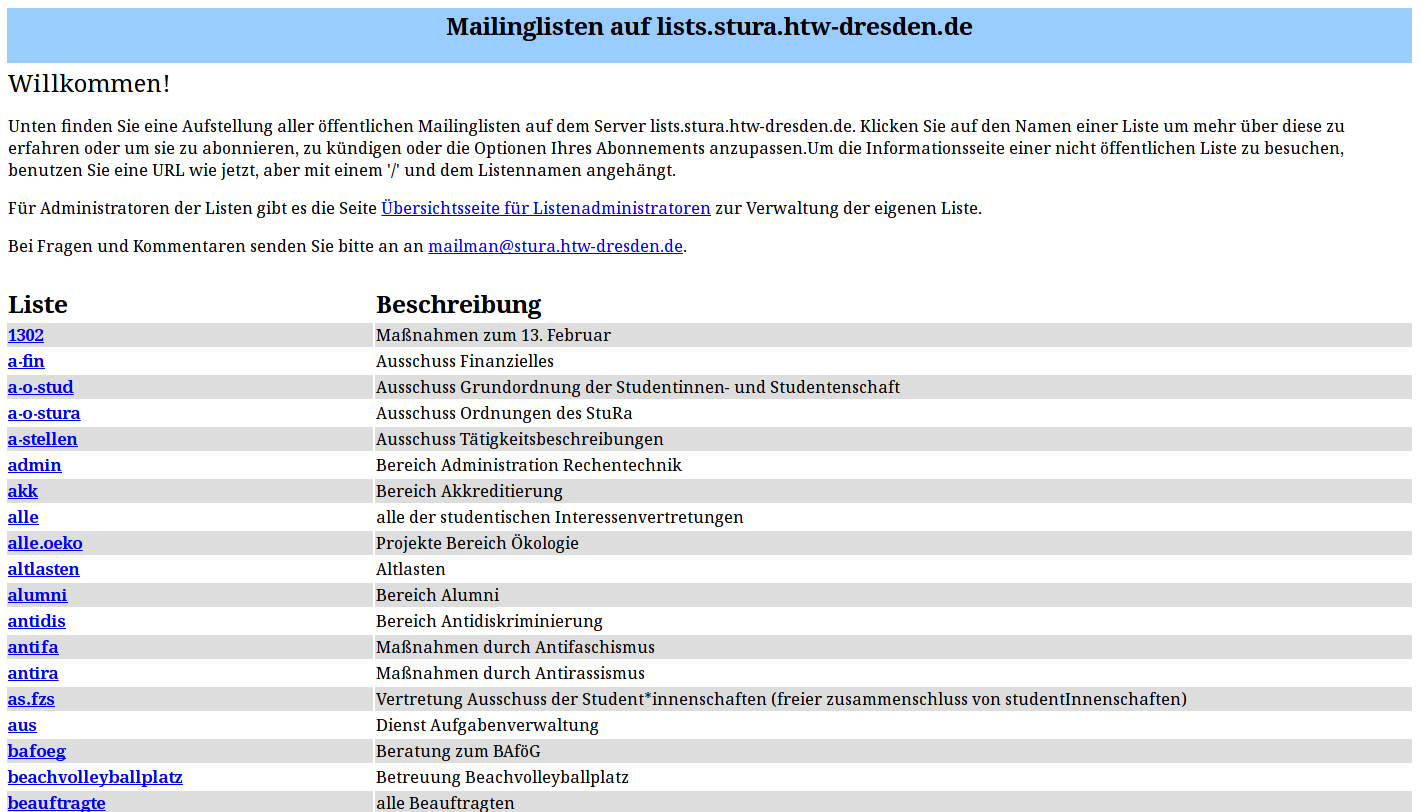
\includegraphics[width=\textwidth]{../images/lists_seite.png}
   \end{figure}

}
%% URL
%% Abbonieren/abbestellen
\subsecframe{Abbonieren} {
	\url{https://lists.stura.htw-dresden.de/listinfo/}\textbf{$<$Name der Liste$>$}
   \begin{figure}
	   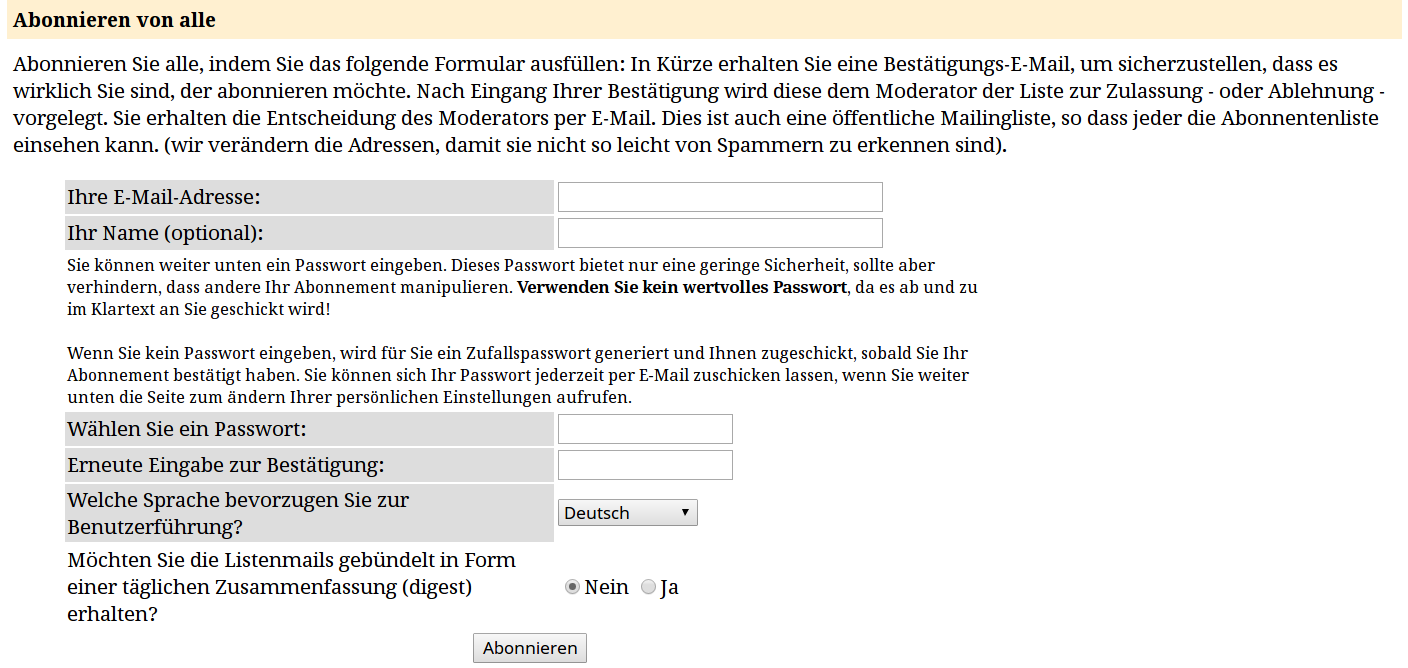
\includegraphics[width=\textwidth]{../images/lists_abbonieren.png}
   \end{figure}
	}
\subsecframe{Optionen} {
	\begin{itemize}
		\item Login f\"ur Mitglieder
		\item K\"undigung des Abos
		\item Passwort zusenden
	\end{itemize}
	\url{https://lists.stura.htw-dresden.de/options/}\textbf{$<$Name der Liste$>$}
	
	}
\frame{
	\frametitle{Login f\"ur Mitglieder}
		Welche E-Mail-Verteiler habe ich abboniert?
   \begin{figure}
	   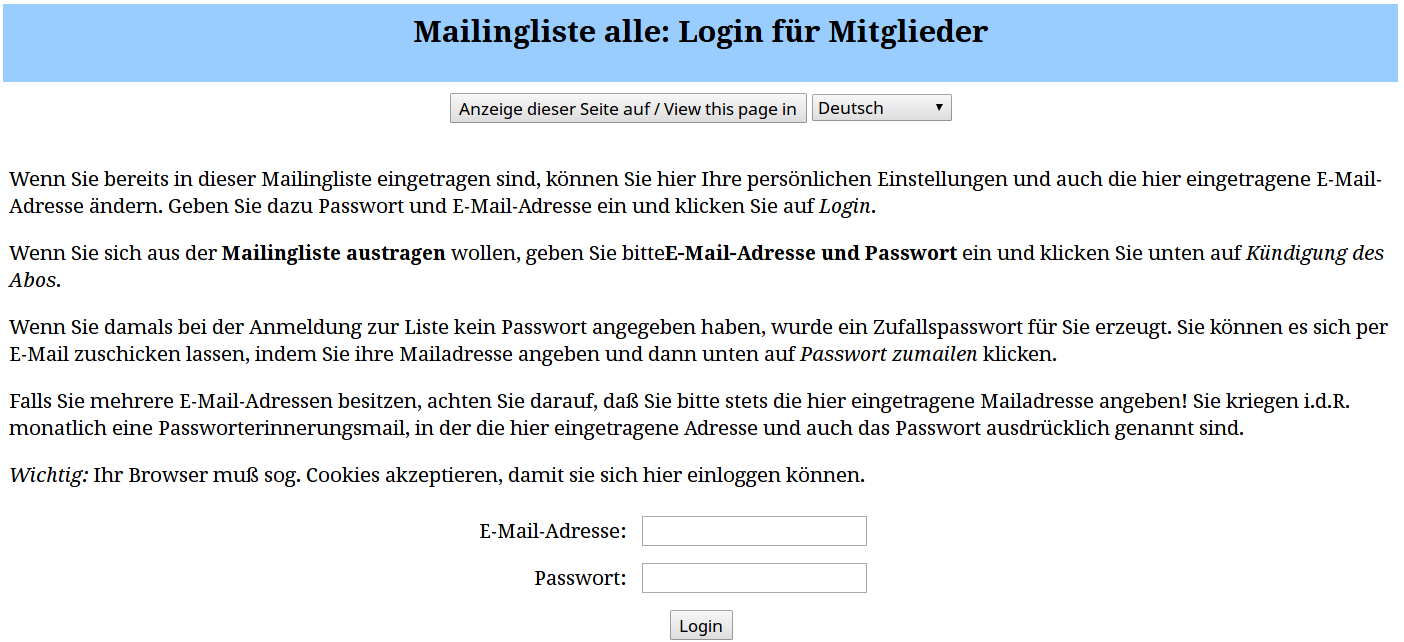
\includegraphics[width=\textwidth]{../images/lists_options.png}
   \end{figure}
   }

\frame{
	\frametitle{K\"undigung des Abos}
	
	M\"ochtest du die Liste abbestellen, dann trage unter \enquote{\textbf{Login f\"ur Mitglieder}} deine E-Mail Adresse und dein Passwort ein und dr\"ucke dann auf \textit{K\"undigung des Abos}.
   \begin{figure}
	   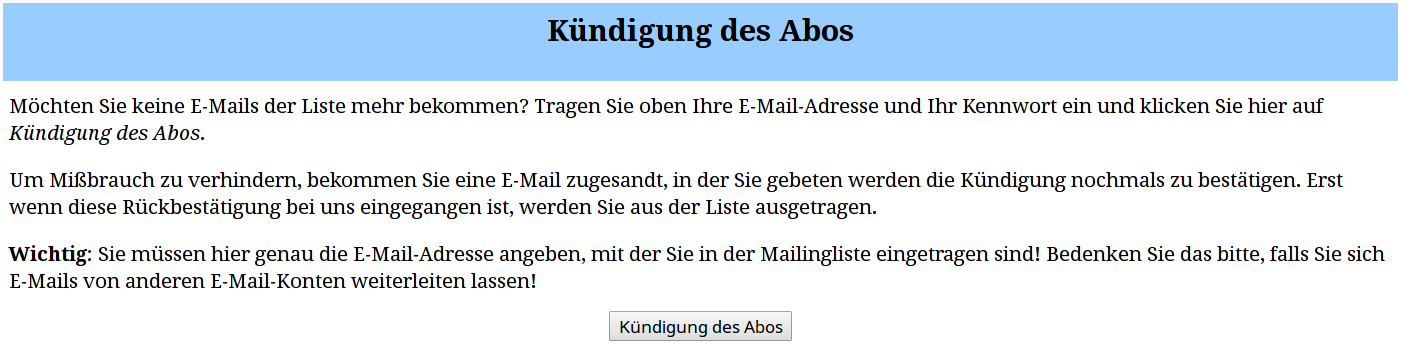
\includegraphics[width=\textwidth]{../images/lists_abbestellen.png}
   \end{figure}
   \begin{hinweis}
   \item Mails von Verteilern haben im Fu{\ss} einen Link auf die Seite unter der die Abmeldung möglich ist.
   \end{hinweis}
	\begin{tip}
	\item Nachfragen an die Administration zur Abmeldung durch Dritte können länger dauern, macht es besser selbst.
	\end{tip}
}
\frame{
	\frametitle{Passwort zusenden}
	Hast du dein Passwort vergessen, dann trage unter \enquote{\textbf{Login f\"ur Mitglieder}} deine E-Mail Adresse ein und dr\"ucke dann auf \enquote{Passwort mailen}.
   \begin{figure}
	   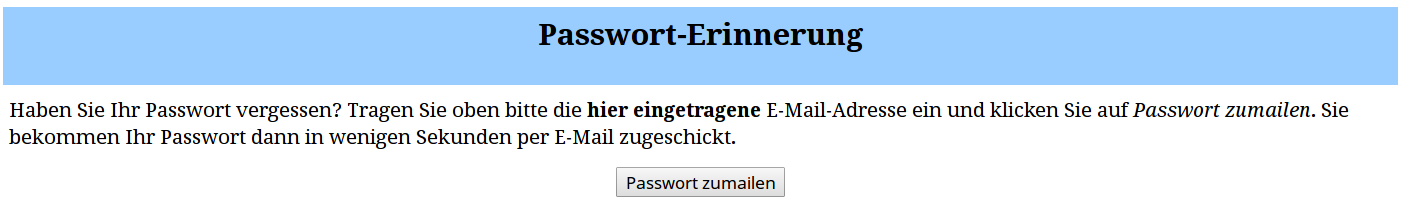
\includegraphics[width=\textwidth]{../images/lists_password_recover.png}
   \end{figure}
}


\frame{
	 Vielen Dank f\"ur Eure Aufmerksamkeit. \\
	\Huge Fragen?
    \begin{minipage}[b]{\linewidth}
\small
    Quellcode: \url{https://github.com/stura-htw-dresden/Basiswissen_E-Mail}
	\end{minipage}
	}

\end{document}
